\documentclass{article}

\usepackage[preprint]{neurips_2026}
\usepackage[utf8]{inputenc}
\usepackage[T1]{fontenc}
\usepackage{hyperref}
\usepackage{url}
\usepackage{booktabs}
\usepackage{tabularx}
\usepackage{array}
\usepackage{amsmath}
\usepackage{amsfonts}
\usepackage{microtype}
\usepackage{xcolor}
\usepackage{graphicx}
\usepackage{tikz}
\usepackage{listings}
\usetikzlibrary{arrows.meta,positioning,calc}

\definecolor{hokBlue}{HTML}{466DB4}
\definecolor{hokTeal}{HTML}{42B4B8}
\definecolor{hokGreen}{HTML}{16845F}
\definecolor{hokOrange}{HTML}{D4742A}
\definecolor{hokRed}{HTML}{B6423C}
\definecolor{hokInk}{HTML}{14213D}
\definecolor{hokMuted}{HTML}{536171}
\definecolor{hokRule}{HTML}{BBCBE5}

\newcommand{\ours}{risk-controlled PPO}
\newcommand{\winrate}{\mathrm{WinRate}}
\newcommand{\towerhp}{\mathrm{TowerHP}}
\newcommand{\death}{\mathrm{Death}}

\lstdefinestyle{appendixcode}{
  basicstyle=\ttfamily\footnotesize,
  breaklines=true,
  columns=fullflexible,
  frame=single,
  framerule=.3pt,
  rulecolor=\color{hokRule},
  backgroundcolor=\color{black!2},
  keywordstyle=\color{hokBlue}\bfseries,
  commentstyle=\color{hokMuted},
  showstringspaces=false,
  tabsize=2
}

\title{Risk-Controlled Tower-Taking for Honor of Kings 1v1 Reinforcement Learning}

\author{%
  Mengfan Liu\\
  Shanghai Innovation Institute\\
  253108110079\\
  \And
  Ditao Li\\
  Shanghai Innovation Institute\\
  253108110078\\
}

\newcommand{\TrainingLoopFigure}{%
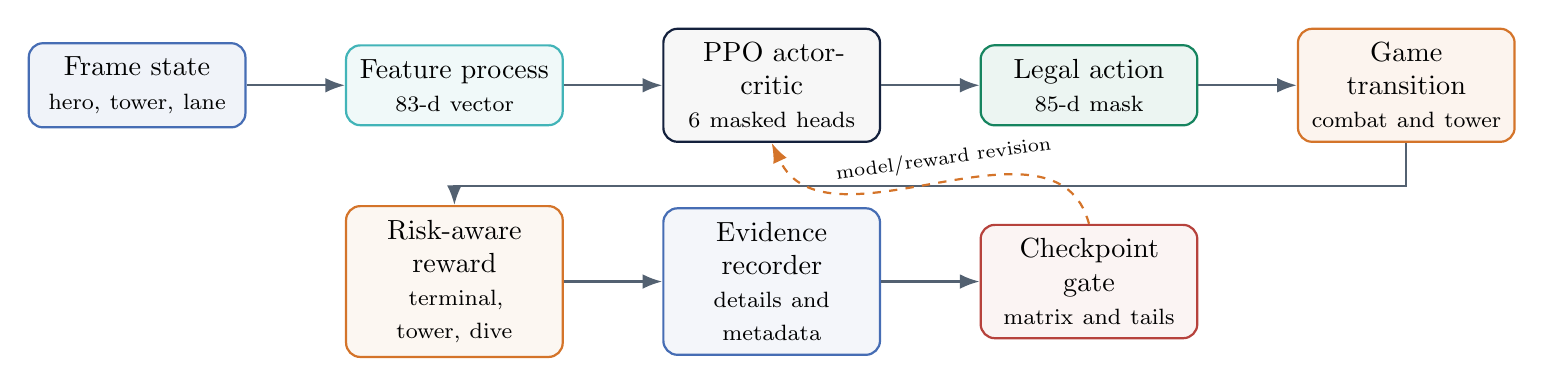
\begin{tikzpicture}[
  node distance=1.25cm,
  >=Latex,
  box/.style={rounded corners=1.8mm, draw, line width=.8pt, align=center,
    inner xsep=5pt, inner ysep=5pt, minimum height=1.0cm, text width=2.4cm},
  flow/.style={-{Latex[length=2.5mm]}, line width=.8pt, draw=hokMuted},
  fb/.style={-{Latex[length=2.5mm]}, line width=.8pt, draw=hokOrange, dashed}
]
  \node[box,draw=hokBlue,fill=hokBlue!8] (state) {Frame state\\{\footnotesize hero, tower, lane}};
  \node[box,draw=hokTeal,fill=hokTeal!8,right=of state] (feat) {Feature process\\{\footnotesize 83-d vector}};
  \node[box,draw=hokInk,fill=black!3,right=of feat] (ppo) {PPO actor-critic\\{\footnotesize 6 masked heads}};
  \node[box,draw=hokGreen,fill=hokGreen!8,right=of ppo] (act) {Legal action\\{\footnotesize 85-d mask}};
  \node[box,draw=hokOrange,fill=hokOrange!8,right=of act] (env) {Game transition\\{\footnotesize combat and tower}};
  \node[box,draw=hokOrange,fill=hokOrange!6,below=1.0cm of feat] (rew) {Risk-aware reward\\{\footnotesize terminal, tower, dive}};
  \node[box,draw=hokBlue,fill=hokBlue!6,right=of rew] (rec) {Evidence recorder\\{\footnotesize details and metadata}};
  \node[box,draw=hokRed,fill=hokRed!6,right=of rec] (sel) {Checkpoint gate\\{\footnotesize matrix and tails}};
  \draw[flow] (state) -- (feat);
  \draw[flow] (feat) -- (ppo);
  \draw[flow] (ppo) -- (act);
  \draw[flow] (act) -- (env);
  \draw[flow] (env.south) -- ++(0,-.55) -| (rew.north);
  \draw[flow] (rew.east) -- (rec.west);
  \draw[flow] (rec.east) -- (sel.west);
  \draw[fb] (sel.north) to[out=105,in=-65] node[pos=.48,above,sloped,font=\scriptsize] {model/reward revision} (ppo.south);
\end{tikzpicture}%
}

\newcommand{\NetworkFigure}{%
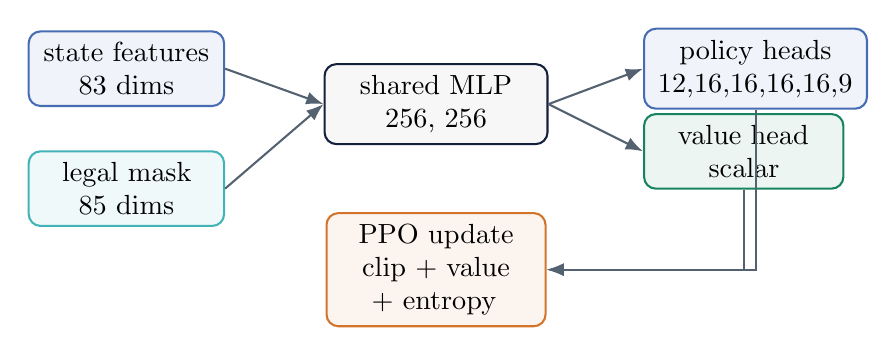
\begin{tikzpicture}[
  >=Latex,
  box/.style={rounded corners=1.5mm, draw, line width=.75pt, align=center,
    inner xsep=4pt, inner ysep=4pt, minimum height=.78cm},
  flow/.style={-{Latex[length=2.2mm]}, line width=.75pt, draw=hokMuted}
]
  \node[box,draw=hokBlue,fill=hokBlue!8,text width=2.2cm] (x) {state features\\83 dims};
  \node[box,draw=hokTeal,fill=hokTeal!8,text width=2.2cm,below=.55cm of x] (m) {legal mask\\85 dims};
  \node[box,draw=hokInk,fill=black!3,text width=2.55cm,right=1.25cm of x,yshift=-.45cm] (enc) {shared MLP\\256, 256};
  \node[box,draw=hokBlue,fill=hokBlue!8,text width=2.55cm,right=1.2cm of enc,yshift=.45cm] (pi) {policy heads\\12,16,16,16,16,9};
  \node[box,draw=hokGreen,fill=hokGreen!8,text width=2.25cm,right=1.2cm of enc,yshift=-.6cm] (v) {value head\\scalar};
  \node[box,draw=hokOrange,fill=hokOrange!8,text width=2.5cm,below=.85cm of enc] (loss) {PPO update\\clip + value + entropy};
  \draw[flow] (x.east) -- (enc.west);
  \draw[flow] (m.east) -- (enc.west);
  \draw[flow] (enc.east) -- (pi.west);
  \draw[flow] (enc.east) -- (v.west);
  \draw[flow] (pi.south) |- (loss.east);
  \draw[flow] (v.south) |- (loss.east);
\end{tikzpicture}%
}

\newcommand{\TrainingCurveFigure}{%
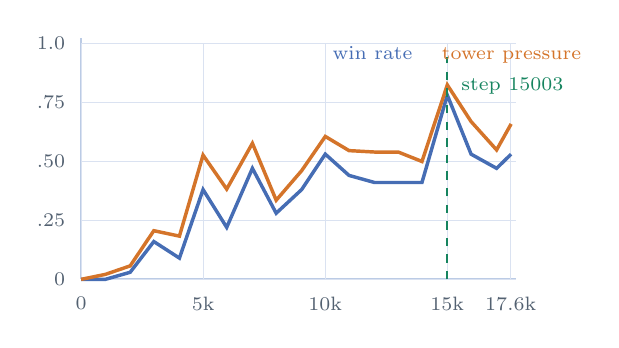
\begin{tikzpicture}[
  x=.31cm,y=3.0cm,
  axis/.style={draw=hokRule,line width=.7pt},
  grid/.style={draw=hokRule!55,line width=.35pt},
  winline/.style={draw=hokBlue,line width=1.25pt},
  towerline/.style={draw=hokOrange,line width=1.25pt},
  tick/.style={font=\scriptsize, color=hokMuted}
]
  \draw[axis] (0,0) -- (17.8,0);
  \draw[axis] (0,0) -- (0,1.02);
  \foreach \y/\lab in {0/0,.25/.25,.5/.50,.75/.75,1/1.0}{
    \draw[grid] (0,\y) -- (17.8,\y);
    \node[anchor=east,tick] at (-.25,\y) {\lab};
  }
  \foreach \x/\lab in {0/0,5/5k,10/10k,15/15k,17.6/17.6k}{
    \draw[grid] (\x,0) -- (\x,1);
    \node[anchor=north,tick] at (\x,-.035) {\lab};
  }
  \draw[winline]
    (0,0) -- (0.992,0) -- (2.010,.03) -- (2.979,.16) -- (4.028,.09) --
    (4.996,.38) -- (5.965,.22) -- (7.018,.47) -- (7.992,.28) --
    (9.035,.38) -- (10.004,.53) -- (10.976,.44) -- (12.023,.41) --
    (12.993,.41) -- (13.964,.41) -- (15.003,.78) -- (15.977,.53) --
    (17.022,.47) -- (17.617,.53);
  \draw[towerline]
    (0,0) -- (0.992,.021) -- (2.010,.057) -- (2.979,.206) -- (4.028,.183) --
    (4.996,.526) -- (5.965,.382) -- (7.018,.576) -- (7.992,.335) --
    (9.035,.460) -- (10.004,.605) -- (10.976,.545) -- (12.023,.539) --
    (12.993,.539) -- (13.964,.499) -- (15.003,.823) -- (15.977,.668) --
    (17.022,.548) -- (17.617,.658);
  \draw[draw=hokGreen,line width=.7pt,dashed] (15.003,0) -- (15.003,.94);
  \node[anchor=west,font=\scriptsize] at (9.9,.95) {\textcolor{hokBlue}{win rate} \quad \textcolor{hokOrange}{tower pressure}};
  \node[anchor=west,font=\scriptsize,color=hokGreen] at (15.18,.82) {step 15003};
\end{tikzpicture}%
}

\newcommand{\CheckpointBars}{%
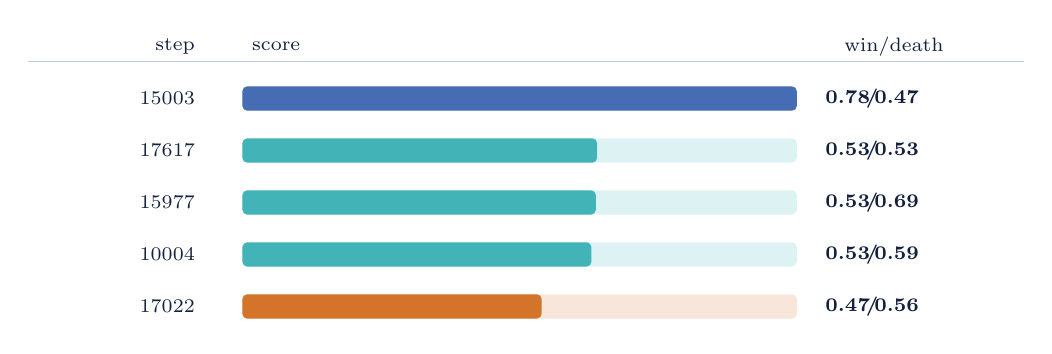
\begin{tikzpicture}[
  x=.08cm,y=.55cm,
  bar/.style={rounded corners=.6mm,draw=none},
  lab/.style={font=\scriptsize,color=hokInk},
  val/.style={font=\scriptsize\bfseries,color=hokInk}
]
  \node[anchor=east,lab] at (28,0) {step};
  \node[anchor=west,lab] at (34,0) {score};
  \node[anchor=west,lab] at (128,0) {win/death};
  \draw[hokRule] (0,-.35) -- (158,-.35);
  \node[anchor=east,lab] at (28,-1.2) {15003};
  \draw[bar,fill=hokBlue!18] (34,-1.48) rectangle (122,-.92);
  \draw[bar,fill=hokBlue] (34,-1.48) rectangle (122,-.92);
  \node[anchor=west,val] at (125,-1.2) {0.78\!/\!0.47};
  \node[anchor=east,lab] at (28,-2.4) {17617};
  \draw[bar,fill=hokTeal!18] (34,-2.68) rectangle (122,-2.12);
  \draw[bar,fill=hokTeal] (34,-2.68) rectangle (90.3,-2.12);
  \node[anchor=west,val] at (125,-2.4) {0.53\!/\!0.53};
  \node[anchor=east,lab] at (28,-3.6) {15977};
  \draw[bar,fill=hokTeal!18] (34,-3.88) rectangle (122,-3.32);
  \draw[bar,fill=hokTeal] (34,-3.88) rectangle (90.1,-3.32);
  \node[anchor=west,val] at (125,-3.6) {0.53\!/\!0.69};
  \node[anchor=east,lab] at (28,-4.8) {10004};
  \draw[bar,fill=hokTeal!18] (34,-5.08) rectangle (122,-4.52);
  \draw[bar,fill=hokTeal] (34,-5.08) rectangle (89.4,-4.52);
  \node[anchor=west,val] at (125,-4.8) {0.53\!/\!0.59};
  \node[anchor=east,lab] at (28,-6.0) {17022};
  \draw[bar,fill=hokOrange!18] (34,-6.28) rectangle (122,-5.72);
  \draw[bar,fill=hokOrange] (34,-6.28) rectangle (81.5,-5.72);
  \node[anchor=west,val] at (125,-6.0) {0.47\!/\!0.56};
\end{tikzpicture}%
}

\begin{document}
\maketitle

\begin{abstract}
This minipaper reports a course-project reinforcement-learning system for the Honor of Kings 1v1 task. The project starts from a PPO agent and redesigns the training loop around the true objective of the environment: converting local lane advantages into tower destruction. We implement an 83-dimensional tactical feature representation, legal-action masking over 6 action branches, terminal and tower-oriented reward terms, explicit push-window and unsafe-dive diagnostics, curriculum hooks, and evidence-driven checkpoint selection. On the available v1.2a evaluation records, the best checkpoint at step 15003 reaches a 0.78 common-AI win rate with 0.47 average deaths, sharply reducing deaths relative to the v1.1 peak while leaving more enemy tower health. The result suggests that risk control is effective but currently under-aggressive; full 9-matchup evaluation is still required before claiming robust generalization.
\end{abstract}

\section{Introduction}

Competitive MOBA reinforcement learning is a useful testbed for sequential decision making because the agent must solve several problems at once: partial observation, long horizons, delayed win signals, high-dimensional state descriptions, and structured action dependencies. Prior Honor of Kings systems demonstrated that actor-critic methods with action masks, scalable training, and carefully shaped objectives can solve complex 1v1 control problems \citep{ye2020moba,wei2022hokarena}. Our project studies a smaller but still instructive version of this setting: a single-agent 1v1 lane task with three marksman heroes, common-AI and self-play opponents, and a final score determined by whether the agent destroys the enemy tower.

The central observation in our development notes is simple but important: the game is not won by maximizing short-term combat. Kills, damage, gold, and forward movement matter only insofar as they create safe tower-taking opportunities. A policy can look active and even achieve high local reward while still failing to finish the tower, or it can learn a high-risk ``trade death for tower damage'' style that works against weak opponents but fails under stronger evaluation. We therefore treat tower-taking as a closed-loop control problem. State features expose tactical windows, the reward function separates objective progress from risk, and checkpoint selection uses evaluation metrics rather than scalar training reward alone.

This paper consolidates the implementation, poster, and optimization documents into a research-style account. The contribution is not a new RL algorithm; instead, it is an auditable engineering recipe for aligning PPO with the 1v1 objective:
\begin{enumerate}
  \item an expanded tactical state encoder covering hero status, towers, lane units, skill availability, tower targets, and relative distances;
  \item a risk-aware reward decomposition with terminal outcome, tower health, push-window tower damage, unsafe-dive penalties, and zero-weight diagnostics;
  \item a training and evaluation pipeline that records configuration snapshots, reward details, opponent schedules, matchup metadata, and checkpoint gates;
  \item an empirical comparison of v1.1 and v1.2a showing that v1.2a greatly compresses deaths but has not yet surpassed the tower pressure of the best v1.1 checkpoint.
\end{enumerate}

\section{Task and system overview}

\paragraph{Environment.}
The task is a 1v1 Honor of Kings lane environment. The controlled hero is sampled from $\{112,133,199\}$, corresponding to Luban, Di Renjie, and Arli in the project configuration. The training workflow iterates through all pairwise hero combinations and supports side switching through the environment configuration. The primary evaluation opponent in the available logs is \texttt{common\_ai}; self-play and historical-opponent schedules are supported by the code but are not fully populated in the v1.2a pulled records.

\paragraph{Objective.}
The official scoring goal is cumulative wins. In this 1v1 map a win is operationally tied to destroying the enemy tower before losing one's own tower or timing out. Consequently, the model-selection objective is not the training reward by itself, but the tuple
\[
  J(\pi)=
  \bigl(\winrate,\; -\towerhp_{\mathrm{enemy}},\; \towerhp_{\mathrm{self}},\; -\death,\; -T\bigr),
\]
where $T$ is episode length. We use this tuple both to explain training behavior and to rank checkpoints.

\begin{figure}[t]
  \centering
  \resizebox{\linewidth}{!}{\TrainingLoopFigure}
  \caption{Closed-loop training architecture. The PPO core is surrounded by tactical feature extraction, risk-aware reward shaping, evidence recording, and checkpoint-gate feedback.}
  \label{fig:loop}
\end{figure}

\paragraph{Code framework.}
The implementation is organized around \texttt{agent\_ppo}. The workflow drives episodes, rotates lineups, injects summoner skills, selects opponents, records metadata, and saves rollout samples. Feature processing is split across hero, tower/organ, and soldier/lane processors. The reward manager computes dense per-frame reward components plus terminal reward at the final frame. The model is a compact actor-critic network with legal-action masking; the algorithm follows clipped PPO \citep{schulman2017ppo} and uses generalized advantage estimation-style rollouts \citep{schulman2016gae}.

\section{Method}

\subsection{Tactical feature representation}

The default baseline feature set was too small for tower-taking decisions. It could observe some hero and enemy-tower state but did not expose enough information about the opposing hero, lane waves, skill readiness, or defensive risk. The current v1.2 implementation uses an 83-dimensional feature vector and an 85-dimensional legal-action vector. Features are normalized whenever possible and are intended to make red/blue-side behavior share a single policy.

The high-value feature groups are shown in Table~\ref{tab:features}. The most important addition for the current research hypothesis is the push-window family: whether allied lane units are near the enemy tower, whether the tower targets a lane unit, whether the agent is within tower range, and whether the enemy hero can punish the approach. These variables allow the reward and diagnostics to distinguish safe tower pressure from unsafe dives.

\begin{table}[t]
  \centering
  \caption{Main feature and signal groups used by the v1.2 PPO agent.}
  \label{tab:features}
  \begin{tabularx}{\linewidth}{>{\bfseries}p{2.8cm}X}
    \toprule
    Group & Examples and purpose \\
    \midrule
    Hero state & hero identity, alive flag, HP/energy, level, experience, economy, attack/defense, movement/attack speed, position, kill/death counters \\
    Enemy state & enemy visibility through state fields, relative position, HP, level/economy differences, revival-related status when available \\
    Skill state & availability and cooldown ratios for attack and skill slots, plus summoner-skill decisions from \texttt{init\_config} \\
    Tower state & self/enemy tower HP, distances to towers, survival, and attack-target indicators \\
    Lane state & nearby allied/enemy soldier count, health mass, push position, and enemy-tower-near wave statistics \\
    Risk/window state & push-window active, unsafe-dive active/severity, low-HP pressure, no-wave tower range, and enemy threat distance \\
    \bottomrule
  \end{tabularx}
\end{table}

\subsection{Actor-critic policy with legal-action masking}

The network is deliberately conservative. A shared MLP maps the 83-dimensional feature vector to two 256-unit hidden layers. Six policy heads produce logits with dimensions $[12,16,16,16,16,9]$, matching the structured action branches. A value head predicts the scalar state value. The legal-action mask is applied inside the PPO loss so that unavailable actions receive no probability mass except for a numerical floor. The code keeps LSTM state fields and 16-step sample formatting for compatibility with the framework, but the current forward pass uses the shared MLP output directly for policy and value prediction.

\begin{figure}[t]
  \centering
  \resizebox{.87\linewidth}{!}{\NetworkFigure}
  \caption{Policy/value architecture. The agent uses a compact shared MLP with six masked action heads and a scalar value head.}
  \label{fig:network}
\end{figure}

For a sampled action branch $a$, PPO optimizes the clipped surrogate objective
\[
  L^{\mathrm{clip}}(\theta)=
  \mathbb{E}_t\left[
  \min\left(r_t(\theta) A_t,\;
  \mathrm{clip}(r_t(\theta),1-\epsilon,1+\epsilon) A_t\right)
  \right],
\]
with $\epsilon=0.2$, $\gamma=0.995$, $\lambda=0.95$, learning rate $5\times10^{-4}$ decaying toward $10^{-4}$, entropy coefficient $0.025$, and gradient clipping at $0.5$. These settings preserve the original PPO backbone while reducing late-training instability relative to the earlier $10^{-3}$ learning-rate setting.

\subsection{Risk-aware reward design}

The v1.2 reward has two design goals. First, it must align dense learning with the sparse terminal objective. Second, it must avoid over-correcting into passive play. Let $\Delta f_i(s_t)$ denote a per-frame difference signal. The reward is decomposed as
\[
R_t =
\sum_i w_i \Delta f_i(s_t)
 + 20\,R_{\mathrm{win}}(s_T)
 + 8\,R_{\mathrm{timeout\ gap}}(s_T).
\]
The configured weights include enemy tower HP decrease ($8.0$), self tower HP loss ($8.0$ as a penalty), tower destruction ($20.0$), hero HP balance ($1.0$), money and experience ($0.5$ each), kill ($2.0$), death ($4.0$ as a penalty), forward progress ($0.05$), push-window tower damage ($2.0$), unsafe-dive indicator ($2.0$), unsafe-dive severity ($1.0$), terminal win/loss ($20.0$), and timeout tower gap ($8.0$). Two diagnostic terms, \texttt{push\_window\_active} and \texttt{unsafe\_dive\_active}, have zero reward weight so they can be logged without changing optimization.

The push-window predicate is true when the hero is close enough to the enemy tower, at least one allied lane unit is near that tower, and the tower is either targeting a lane unit or the enemy hero is dead/far away. The unsafe-dive severity grows when the agent is in tower range with no allied wave, low HP, tower aggro, or a nearby live enemy. This makes the reward distinguish a good tower hit from a visually similar but strategically bad overextension.

\subsection{Training curriculum and evidence logging}

The workflow records a configuration snapshot at training start, including reward profile, reward-weight overrides, opponent schedule, model pool, and relevant TOML files. Each episode record contains lineup, side, evaluation flag, opponent source, checkpoint snapshot, and user configuration. The design supports common-AI anchoring, historical checkpoint opponents, and latest self-play. In v1.2a, the analysis focuses on common-AI records because self-play and reward-detail metrics were missing in the available pulled logs.

This evidence-first structure is central to the project. Since PPO reward can diverge from the actual game objective, the selected checkpoint should be the one that best satisfies the evaluation tuple, not necessarily the final or highest-reward checkpoint.

\section{Experiments}

\paragraph{Baselines and variants.}
The main comparison is between v1.1 and v1.2a. v1.1 expanded features from the minimal starter set to 63 dimensions, fixed summoner-skill selection, introduced tower/hero/economy rewards, and reached a strong common-AI peak. v1.2a further expands features to 83 dimensions, adds terminal rewards, splits tower reward terms, introduces push-window and unsafe-dive shaping, lowers the learning rate, and adds evidence tools for checkpoint selection and ablations.

\paragraph{Metrics.}
We report common-AI win rate, enemy tower HP, self tower HP, average frame count, kill/death, money per frame, hero damage dealt/taken, and scalar training reward. For checkpoint ranking, the project tool combines win rate, death, enemy tower HP, and hero-damage balance. For final validation, the planned matrix requires all 9 hero matchups, side swaps, sufficient repeats, p90 death, p10 self-tower HP, timeout rate, push-window tower-damage share, and unsafe-dive/death correlation.

\paragraph{Ablation plan.}
The implementation exposes reward profiles for clean ablations: \texttt{no\_window\_reward} removes push-window and unsafe-dive shaping, \texttt{no\_terminal\_reward} removes terminal win and timeout tower-gap rewards, and \texttt{death\_only\_risk} keeps death/severity risk while removing window and self-tower shaping. These profiles are not yet fully evaluated in the available logs, but they make the research claims testable without manual code edits.

\section{Results}

\subsection{Training dynamics}

Figure~\ref{fig:curve} summarizes v1.2a common-AI training dynamics. The run has a cold-start phase, a first breakthrough around 5k--7k steps, a plateau from roughly 8k--14k, a sharp peak at step 15003, and then regression in gameplay metrics even as scalar reward later improves. This is exactly why checkpoint selection must be metric-driven.

\begin{figure}[t]
  \centering
  \resizebox{.88\linewidth}{!}{\TrainingCurveFigure}
  \caption{v1.2a common-AI win rate and tower pressure. Tower pressure is $1-\mathrm{enemy\ tower\ HP}/12000$. Step 15003 is the strongest gameplay checkpoint.}
  \label{fig:curve}
\end{figure}

\begin{table}[t]
  \centering
  \caption{Key checkpoint comparison from project logs. Lower death is better; lower enemy tower HP is better.}
  \label{tab:results}
  \begin{tabular}{lrrrrrr}
    \toprule
    Checkpoint & Win & Enemy tower HP & Self tower HP & Frame & Kill & Death \\
    \midrule
    v1.1 step 15000 & 0.84 & 1401 & 7745 & 13670 & 3.75 & 2.72 \\
    v1.1 step 17057 & 0.75 & 1252 & 6690 & 13617 & 3.41 & 3.09 \\
    v1.2a step 15003 & 0.78 & 2129 & 4296 & 15726 & 3.44 & 0.47 \\
    v1.2a step 17617 & 0.53 & 4106 & 3346 & 14609 & 3.03 & 0.53 \\
    \bottomrule
  \end{tabular}
\end{table}

\subsection{Checkpoint selection}

The v1.2a ranking tool recommends step 15003. It is the only available checkpoint that combines high common-AI win rate, strong tower pressure, low death, and acceptable hero-damage balance. The final checkpoint, step 17617, has better scalar reward but worse gameplay: win rate drops to 0.53 and enemy tower HP rises to 4106. This mismatch supports the paper's central engineering claim: scalar reward is a learning signal, not a sufficient model-selection criterion.

\begin{figure}[t]
  \centering
  \resizebox{.82\linewidth}{!}{\CheckpointBars}
  \caption{Top v1.2a checkpoint ranking. The recommended step 15003 has the best composite score and a 0.78/0.47 win/death profile.}
  \label{fig:rank}
\end{figure}

\subsection{Interpretation}

Relative to v1.1 step 15000, v1.2a step 15003 loses 0.06 win rate and leaves about 729 more enemy tower HP, but reduces average deaths by 2.25. This is a large behavioral shift. The agent is much safer, but safety has not yet been converted into faster tower wins. The most likely explanation is over-correction: risk terms and lower learning rate reduce deaths and incoming damage, while objective pressure is still insufficient to match v1.1's tower conversion.

The candidate gate therefore marks v1.2a step 15003 as promising but not final. It passes death and explicit-checkpoint-selection criteria, warns on win rate and enemy tower HP, and marks matchup coverage, push-window evidence, death-tail risk, self-tower tail risk, timeout rate, and unsafe-dive diagnostics as missing. This is a useful scientific outcome: the project can now state what improved, what regressed, and what evidence is required next.

\section{Discussion and limitations}

The project demonstrates that a research-like loop can be built on top of a course PPO implementation. Instead of repeatedly training and hoping the latest checkpoint is best, the workflow now encodes hypotheses, exposes reward profiles for ablation, records evidence, and ranks checkpoints by task metrics. The main positive result is death compression: v1.2a shows that explicit risk modeling can change behavior substantially. The main negative result is objective under-conversion: lower death alone does not guarantee better tower-taking.

Several limitations remain. First, the v1.2a records used here contain only common-AI evaluation summaries and lack complete reward-detail diagnostics. Second, the full 9-matchup matrix is not yet available, so the strongest claim is about the observed common-AI aggregate, not robust cross-hero generalization. Third, although the data pipeline formats 16-step recurrent samples, the current model forward path does not exploit the LSTM output for policy/value computation; temporal modeling remains future work. Fourth, reward weights were chosen by engineering judgment and should be validated through controlled ablations.

The next iteration should keep the death reduction but restore objective pressure. Concretely, we recommend evaluating step 15003 on the fixed matchup matrix, increasing tower-conversion incentives only after reward-detail logging is verified, and comparing the three configured reward ablations. If push-window features improve tower damage share without raising death tails, the tactical-window hypothesis is supported. If the death-only profile is safe but weak, the results would confirm that risk control must be coupled to objective opportunity modeling.

\section{Conclusion}

We presented a risk-controlled PPO agent for Honor of Kings 1v1 tower-taking. The system combines tactical feature expansion, action masking, terminal and tower-aware rewards, push-window and unsafe-dive modeling, curriculum hooks, and evidence-driven checkpoint selection. The best observed v1.2a checkpoint reaches 0.78 common-AI win rate with only 0.47 deaths, indicating strong safety gains but incomplete tower conversion. The minipaper's main conclusion is therefore balanced: v1.2a is a credible candidate and a better experimental platform, but a final model claim requires matchup-matrix evaluation and reward-mechanism diagnostics.

\section*{References}
\begin{thebibliography}{9}

\bibitem[Berner et~al.(2019)]{berner2019dota}
Christopher Berner, Greg Brockman, Brooke Chan, Vicki Cheung, Przemyslaw Debiak,
Christy Dennison, David Farhi, Quirin Fischer, Shariq Hashme, Chris Hesse,
Rafal Jozefowicz, Scott Gray, Catherine Olsson, Jakub Pachocki, Michael Petrov,
Henrique~Pondé de~Oliveira~Pinto, Jonathan Raiman, Tim Salimans, Jeremy Schlatter,
Jonas Schneider, Szymon Sidor, Ilya Sutskever, Jie Tang, Filip Wolski, and Susan Zhang.
\newblock Dota 2 with large scale deep reinforcement learning.
\newblock \emph{arXiv preprint arXiv:1912.06680}, 2019.

\bibitem[Schulman et~al.(2016)]{schulman2016gae}
John Schulman, Philipp Moritz, Sergey Levine, Michael Jordan, and Pieter Abbeel.
\newblock High-dimensional continuous control using generalized advantage estimation.
\newblock In \emph{International Conference on Learning Representations}, 2016.

\bibitem[Schulman et~al.(2017)]{schulman2017ppo}
John Schulman, Filip Wolski, Prafulla Dhariwal, Alec Radford, and Oleg Klimov.
\newblock Proximal policy optimization algorithms.
\newblock \emph{arXiv preprint arXiv:1707.06347}, 2017.

\bibitem[Vinyals et~al.(2019)]{vinyals2019alphastar}
Oriol Vinyals, Igor Babuschkin, Wojciech~M. Czarnecki, Michaël Mathieu, Andrew Dudzik,
Junyoung Chung, David~H. Choi, Richard Powell, Timo Ewalds, Petko Georgiev, and others.
\newblock Grandmaster level in StarCraft II using multi-agent reinforcement learning.
\newblock \emph{Nature}, 575:350--354, 2019.

\bibitem[Wei et~al.(2022)]{wei2022hokarena}
Hua Wei, Jingxiao Chen, Xiyang Ji, Hongyang Qin, Minwen Deng, Siqin Li, Liang Wang,
Weinan Zhang, Yong Yu, Lin Liu, Lanxiao Huang, Deheng Ye, Qiang Fu, and Wei Yang.
\newblock Honor of Kings Arena: an environment for generalization in competitive reinforcement learning.
\newblock In \emph{Advances in Neural Information Processing Systems}, volume 35, pages 11881--11892, 2022.

\bibitem[Ye et~al.(2020)]{ye2020moba}
Deheng Ye, Zhao Liu, Mingfei Sun, Bei Shi, Peilin Zhao, Hao Wu, Hongsheng Yu,
Shaojie Yang, Xipeng Wu, Qingwei Guo, Qiaobo Chen, Yinyuting Yin, Hao Zhang,
Tengfei Shi, Liang Wang, Qiang Fu, Wei Yang, and Lanxiao Huang.
\newblock Mastering complex control in MOBA games with deep reinforcement learning.
\newblock In \emph{Proceedings of the AAAI Conference on Artificial Intelligence},
volume 34, pages 6672--6679, 2020.

\end{thebibliography}

\appendix
\section{Implementation checklist}

\begin{table}[h]
  \centering
  \caption{Files that instantiate the paper's main components.}
  \begin{tabularx}{\linewidth}{>{\ttfamily}p{3.2cm}X}
    \toprule
    File & Role \\
    \midrule
    conf.py & feature/action dimensions, PPO hyperparameters, reward profiles and weights \\
    model.py & shared MLP actor-critic network, masked PPO loss, entropy/value terms \\
    reward\_process.py & tower, terminal, push-window, unsafe-dive, and diagnostic reward logic \\
    train\_workflow.py & lineup rotation, opponent schedule, episode loop, terminal reward insertion, evidence logging \\
    select\_checkpoint.py & metric-driven checkpoint ranking \\
    evaluation\_matrix.py & planned checkpoint by matchup by side-swap evaluation design \\
    \bottomrule
  \end{tabularx}
\end{table}

\section{Representative code excerpt}

The project keeps the reward hypothesis executable through named profiles and compact tactical predicates. The excerpt below is adapted from \texttt{agent\_ppo/conf/conf.py} and \texttt{agent\_ppo/feature/reward\_process.py}; it illustrates how the minipaper's terminal, tower-window, and unsafe-dive claims are connected to actual code.

\begin{lstlisting}[style=appendixcode,language=Python]
BASE_REWARD_WEIGHT_DICT = {
    "enemy_tower_hp_down": 8.0,
    "self_tower_hp_down": 8.0,
    "tower_destroy": 20.0,
    "death": 4.0,
    "push_window_tower_damage": 2.0,
    "unsafe_dive": 2.0,
    "unsafe_dive_severity": 1.0,
    "win_result": 20.0,
    "timeout_tower_gap": 8.0,
}

REWARD_PROFILE_OVERRIDES = {
    "no_window_reward": {
        "push_window_tower_damage": 0.0,
        "unsafe_dive": 0.0,
        "unsafe_dive_severity": 0.0,
    },
    "no_terminal_reward": {
        "win_result": 0.0,
        "timeout_tower_gap": 0.0,
    },
}

def _has_push_window(self, main_hero, enemy_hero, enemy_tower, frame_data, camp):
    near_wave_count = self._nearby_lane_count(frame_data, camp, enemy_tower)
    tower_targets_wave = self._tower_targets_lane_unit(frame_data, camp, enemy_tower)
    hero_close = self._distance(main_hero, enemy_tower) <= TOWER_WINDOW_DISTANCE
    enemy_far_or_dead = (
        enemy_hero is None
        or enemy_hero.get("hp", 0) <= 0
        or self._distance(main_hero, enemy_hero) > HERO_THREAT_DISTANCE
    )
    return hero_close and near_wave_count > 0 and (tower_targets_wave or enemy_far_or_dead)
\end{lstlisting}

\section{Minimum final-evaluation protocol}

The project should not claim a final robust agent until the following protocol is run for the selected checkpoint: all $3\times3$ hero matchups; blue/red side swaps; at least 20 repeats per matchup; fixed summoner-skill policy or a separately reported skill grid; common-AI, historical-checkpoint, and self-play opponent slices; and a report containing average and worst-matchup win rate, enemy tower HP, self tower HP, frame count, death mean and p90, self-tower HP p10, timeout rate, push-window tower-damage share, and unsafe-dive/death correlation.

\section{Reward-profile ablations}

\begin{table}[h]
  \centering
  \caption{Planned ablations for validating the mechanism-level story.}
  \begin{tabularx}{\linewidth}{>{\ttfamily}p{3.2cm}X}
    \toprule
    Profile & Interpretation if performance drops \\
    \midrule
    v1.2 & Full recipe: terminal, tower, push-window, and unsafe-dive terms \\
    no\_window\_reward & Tests whether tactical-window modeling improves objective conversion beyond generic tower reward \\
    no\_terminal\_reward & Tests whether direct win/loss alignment is required for checkpoint quality \\
    death\_only\_risk & Tests whether safety alone is too conservative without tower-window opportunity modeling \\
    \bottomrule
  \end{tabularx}
\end{table}

\end{document}
